\documentclass{article}
\usepackage[utf8]{inputenc}
\usepackage[margin=0.7in]{geometry}
\usepackage{amsmath,amssymb}
\usepackage{graphicx}

\newcommand{\pin}{p^{\mathrm{in}}}
\newcommand{\pout}{p^{\mathrm{out}}}
\newcommand{\Pout}{P_{\mathrm{out}}}
\newcommand{\kin}{\langle k \rangle^{\mathrm{in}}}
\newcommand{\kout}{\langle k \rangle^{\mathrm{out}}}
\newcommand{\meank}{\langle k \rangle}
\newcommand{\meanS}{\langle s \rangle}

%\input{figures}

\begin{document}

\section{Model}

Parameters:

\begin{itemize}
\item $N$: Network size
\item $N_c$: Number of nodes per block
\item $\ell$: Number of blocks
\item $\meank$: Average degree of the overall network
\item $\kin$: Average degree counting only intrablock links
\item $\kout$: Average degree counting only interblock links
\item $\pin$: Probability of existence of intrablock links
\item $\pout$: Probability of existence of interblock links
\end{itemize}

Relation between parameters:

\begin{align}
N &= \ell N_c \\
\meank &= \kin + \kout =  \pin (N_c - 1) + \pout (N - N_c)\\
N_r &= N/N_c\\
\Pout &= \pout N_c^2
\end{align}


\section{Results}

It seems that the effective size of the system is not the number of nodes $N$ but the ratio between $N$ and the size of the blocks. Thus, we define the variable $N_r = N/N_c$ and perform the analysis in terms of this variable.

For constant $N_c$ and  $\meank$ large enough ($\meank \gtrsim 4$), the transition occurs when 

\begin{equation}
N_r \Pout = 1,
\end{equation}

where $\Pout = \pout N_c^2$ is the average number of links connecting two given blocks. For smaller values of $\meank$, the percolation point moves to the right, as it can be seen in Figures \ref{fig:scaling} and \ref{fig:perc_point}. The critical exponents do not seem to vary.

\textbf{Hipothesis:} the (finite-size) percolation threshold and the peak of $N_2$ and $\meanS$, for a given value of $N$, satisfy a scaling relation of the type

\begin{align}
q_c(N, \meank) - q_c(N, \meank_{\mathrm{max}}) &\sim \meank^a \\
\dfrac{1}{N_2^{\mathrm{max}}(N, \meank)} - \mathrm{const} &\sim \meank^b \\
\dfrac{1}{\meanS^{\mathrm{max}}(N, \meank)} - \mathrm{const} &\sim \meank^c
\end{align}

\begin{figure}
\centering
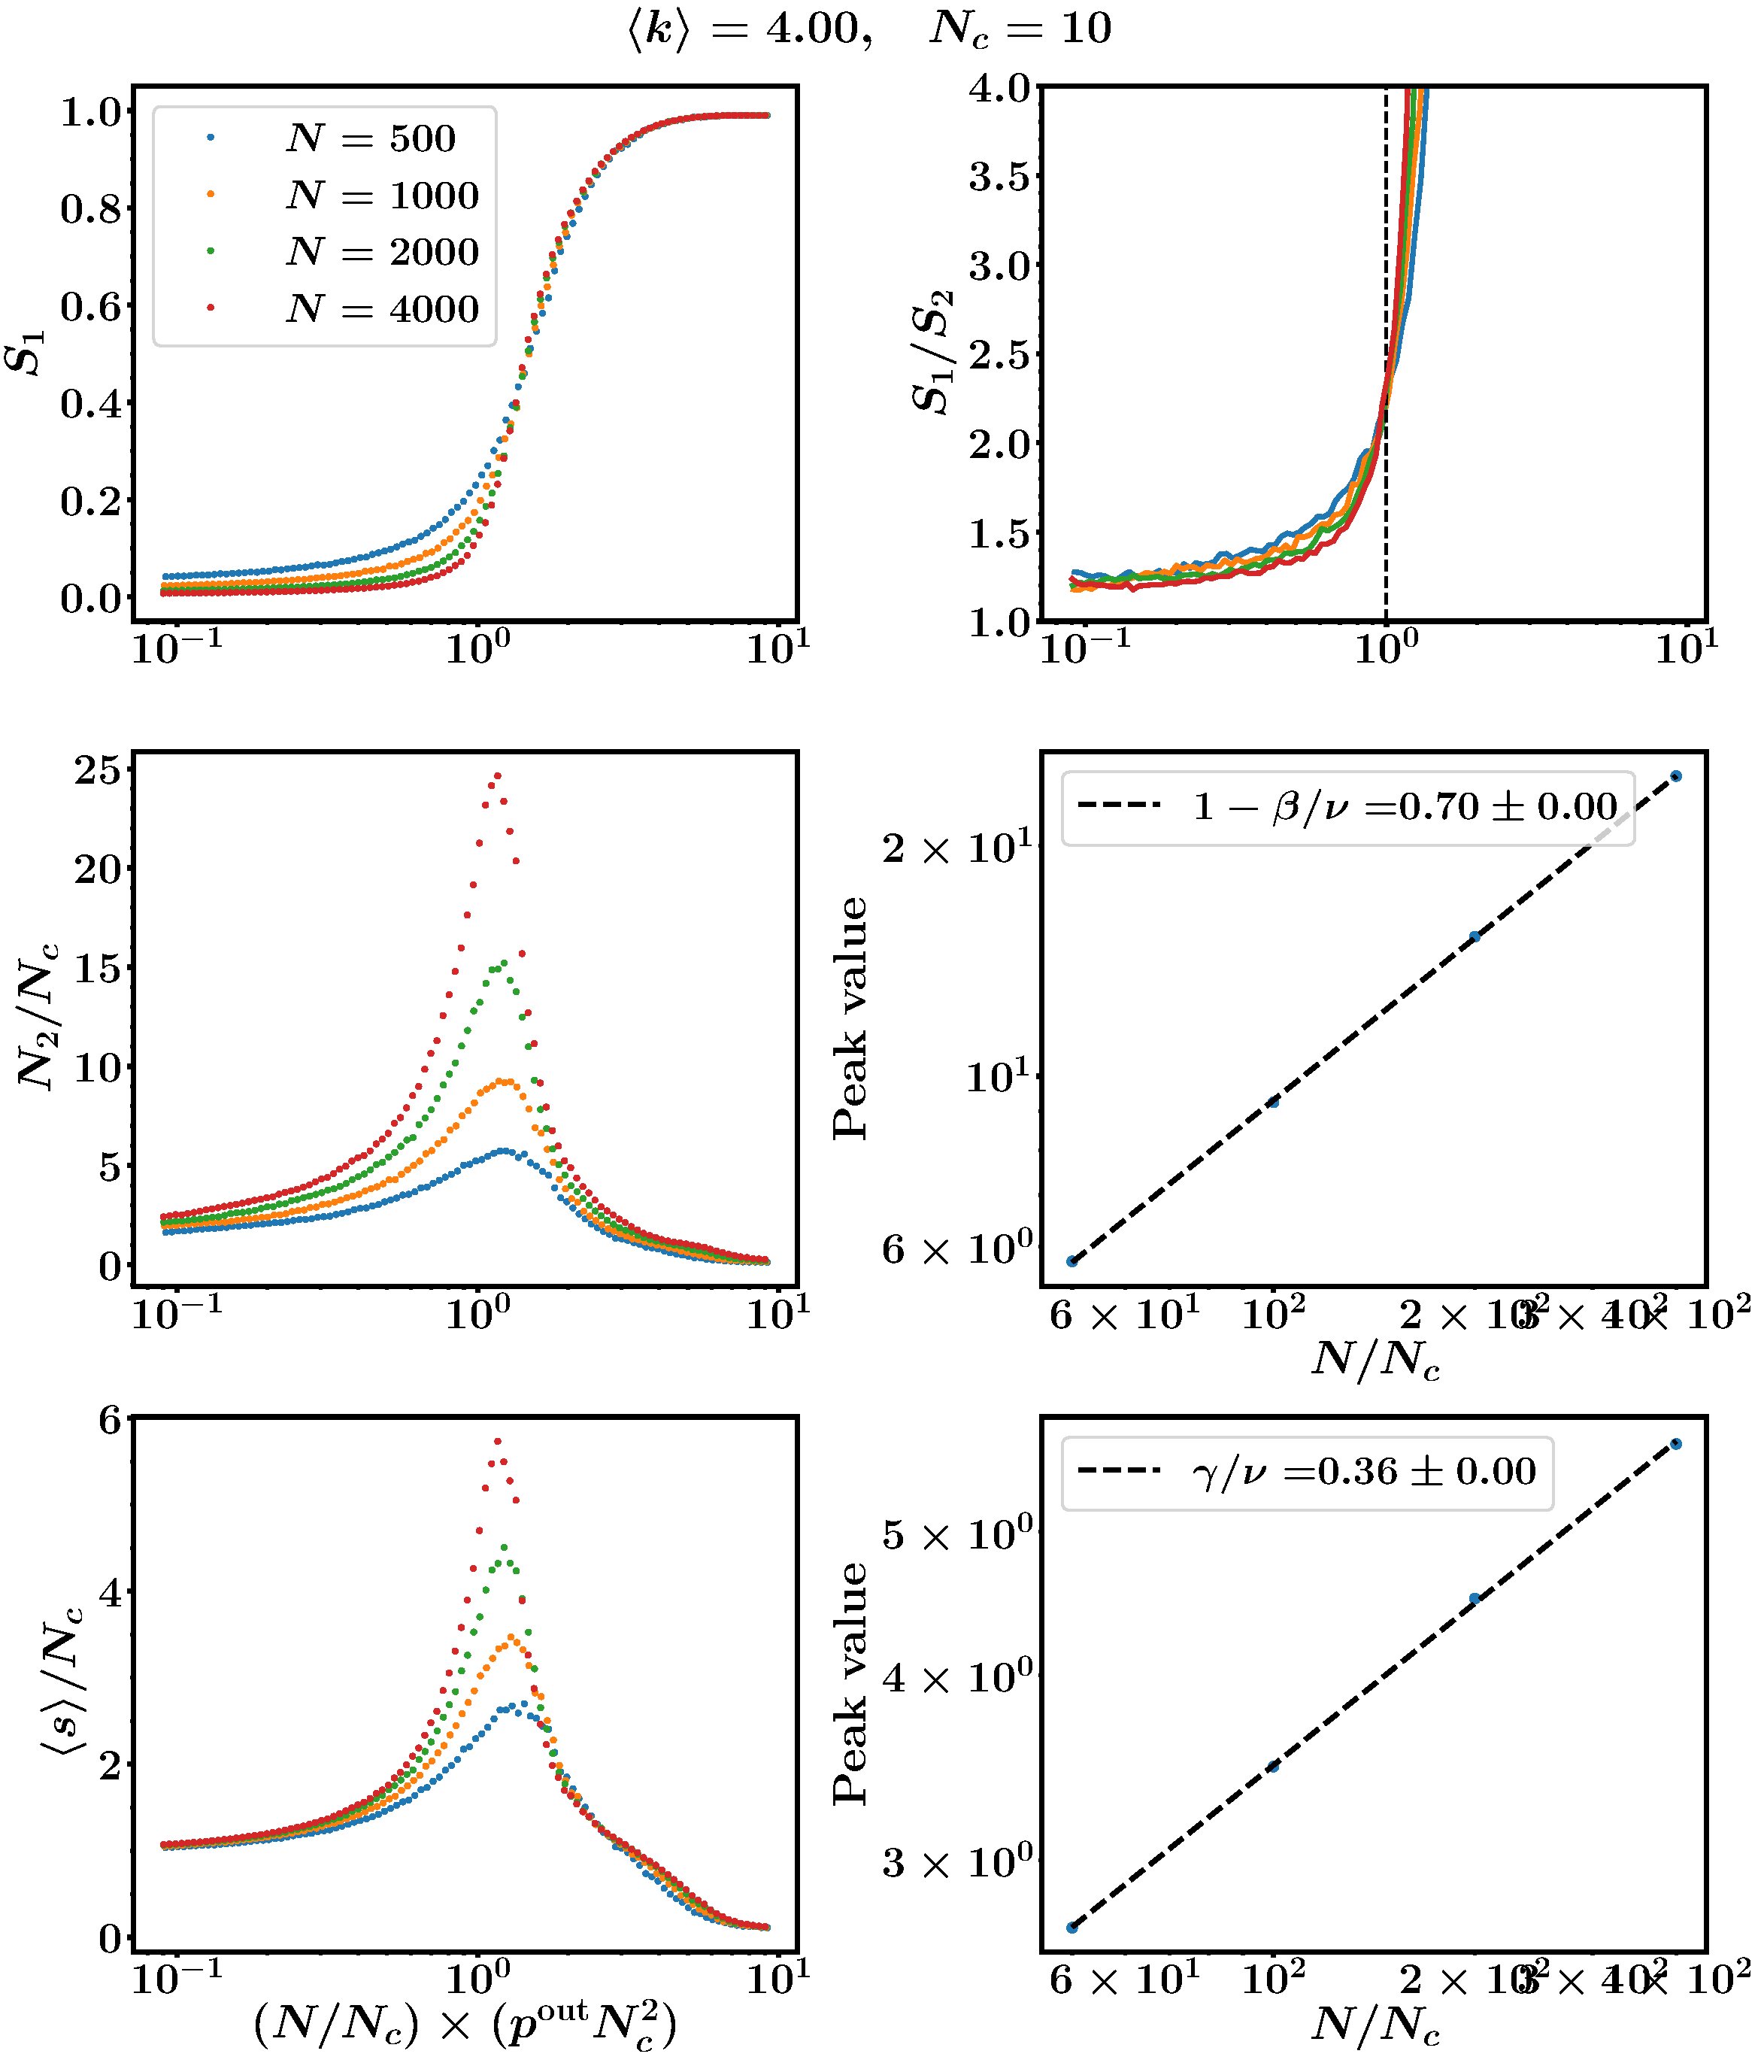
\includegraphics[scale=0.24]{{figures/scaling_k4.00_Nc10_it1000_samples100_Log}.pdf}%
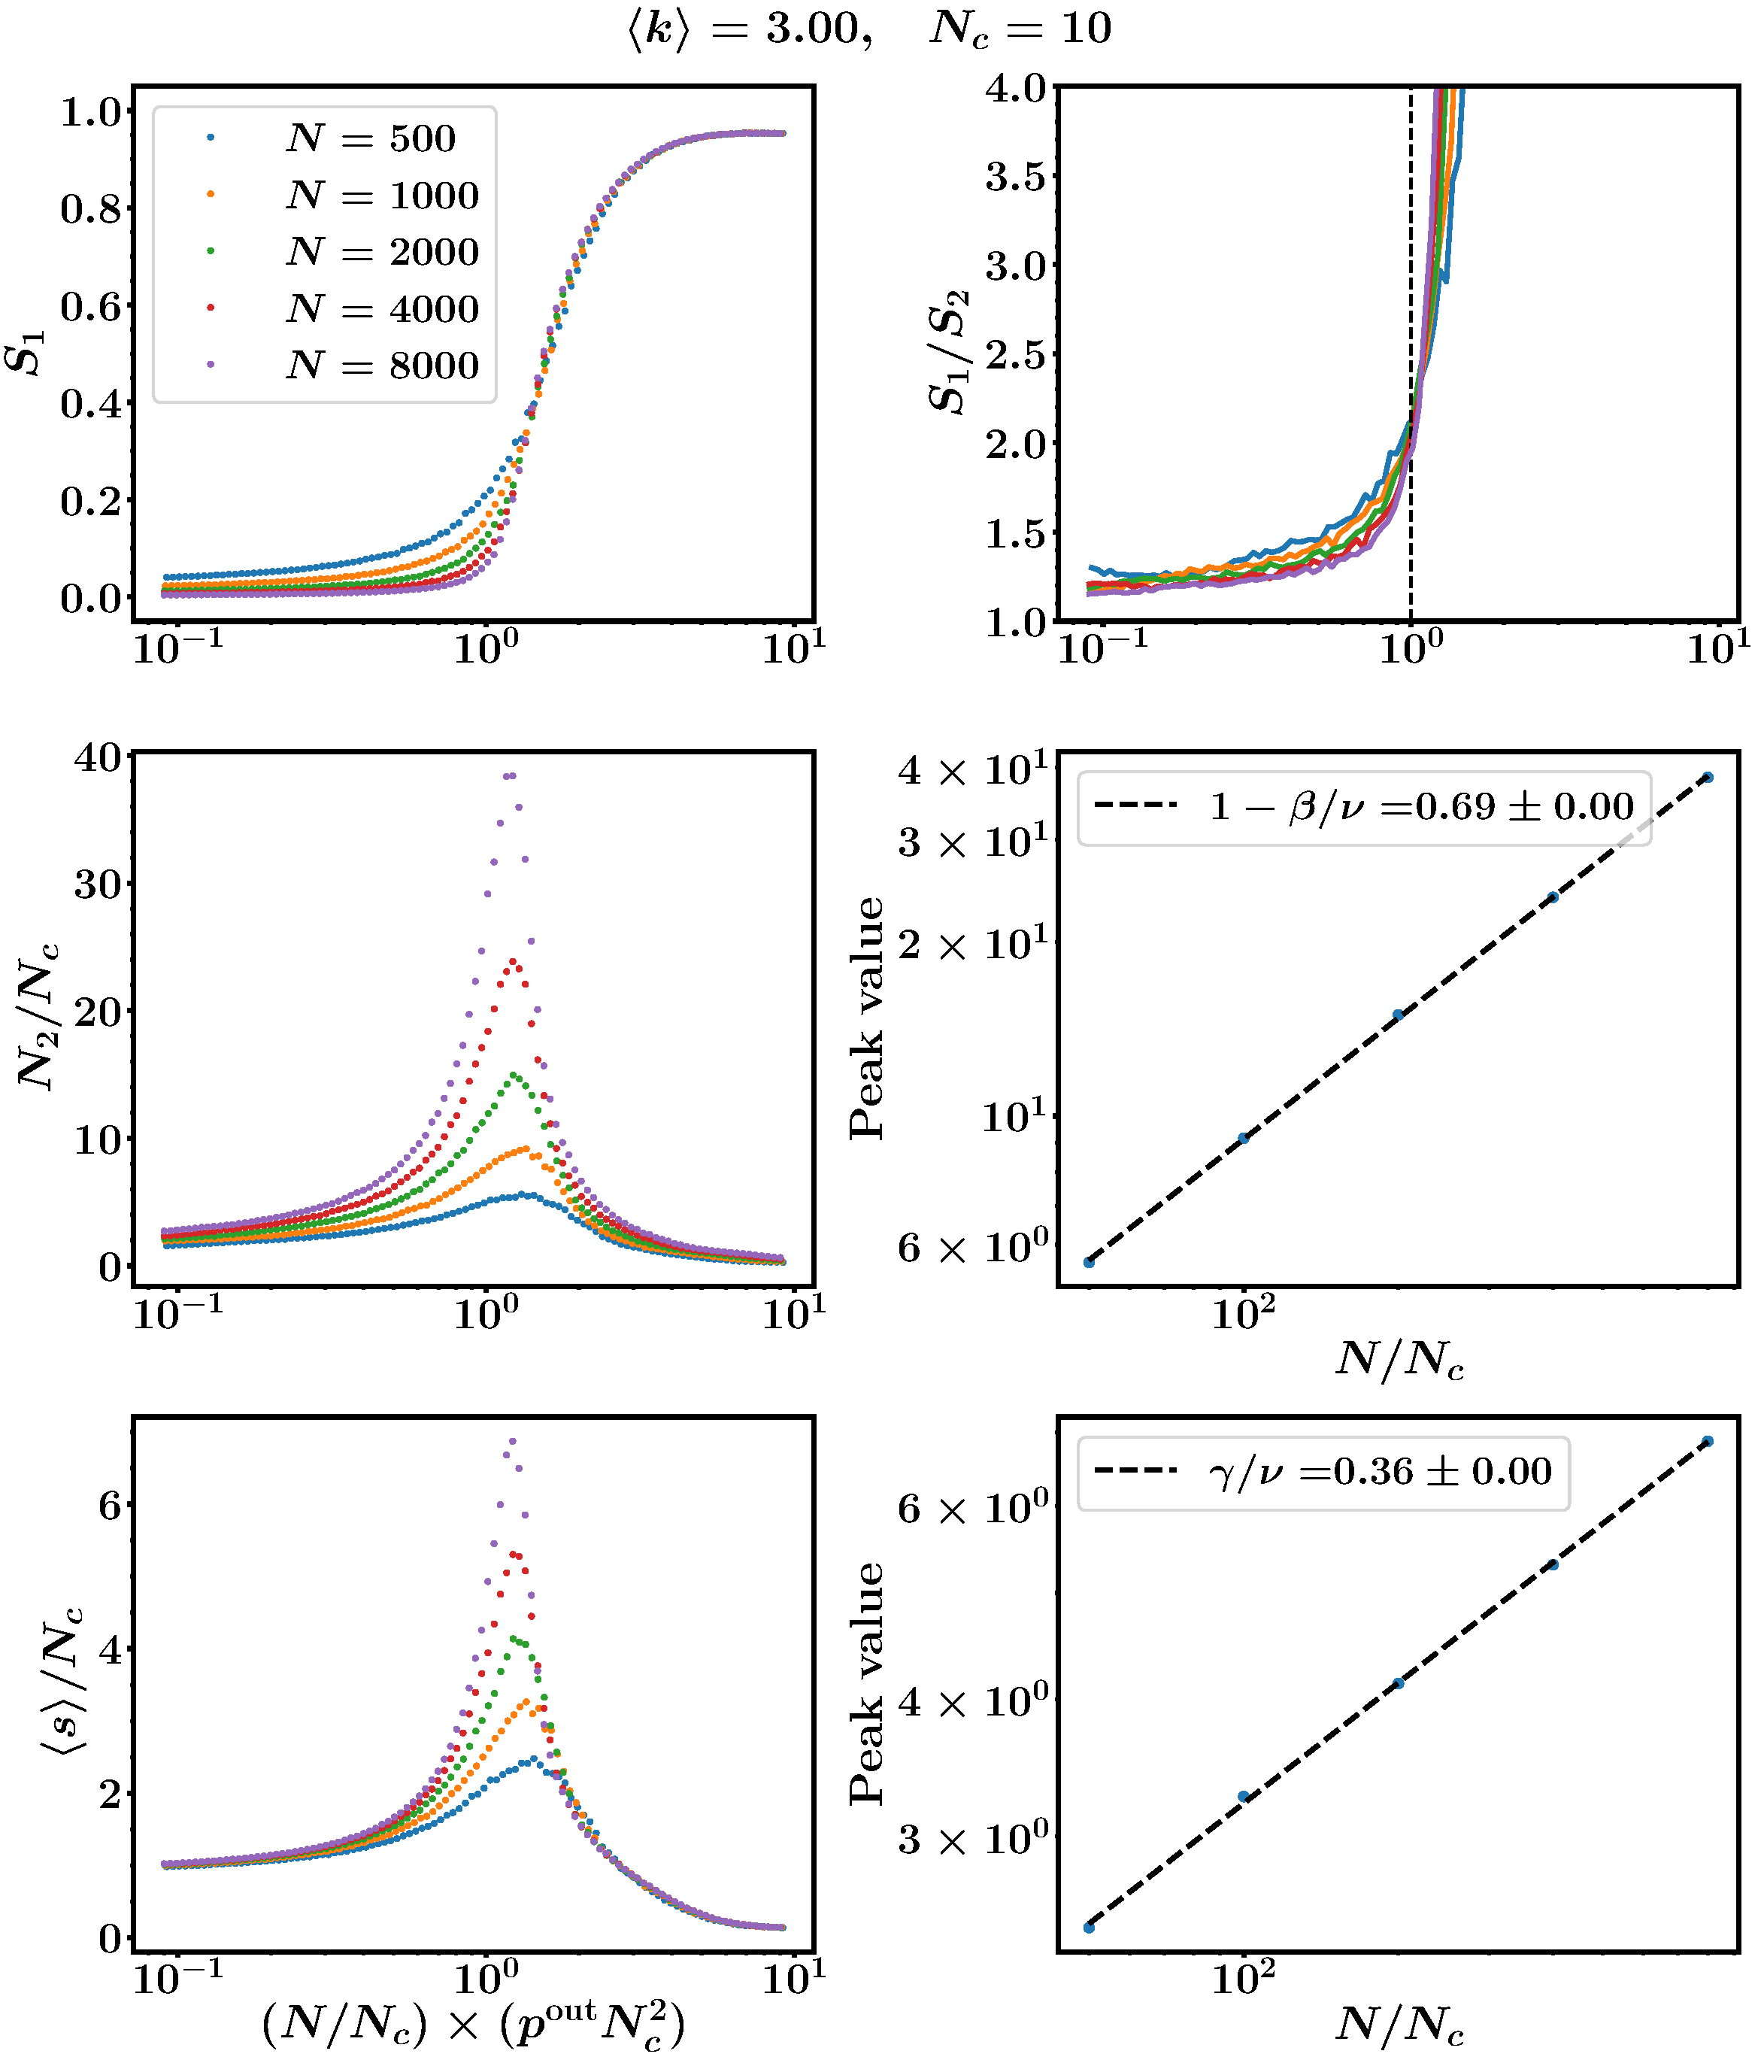
\includegraphics[scale=0.24]{{figures/scaling_k3.00_Nc10_it1000_samples100_Log}.pdf}
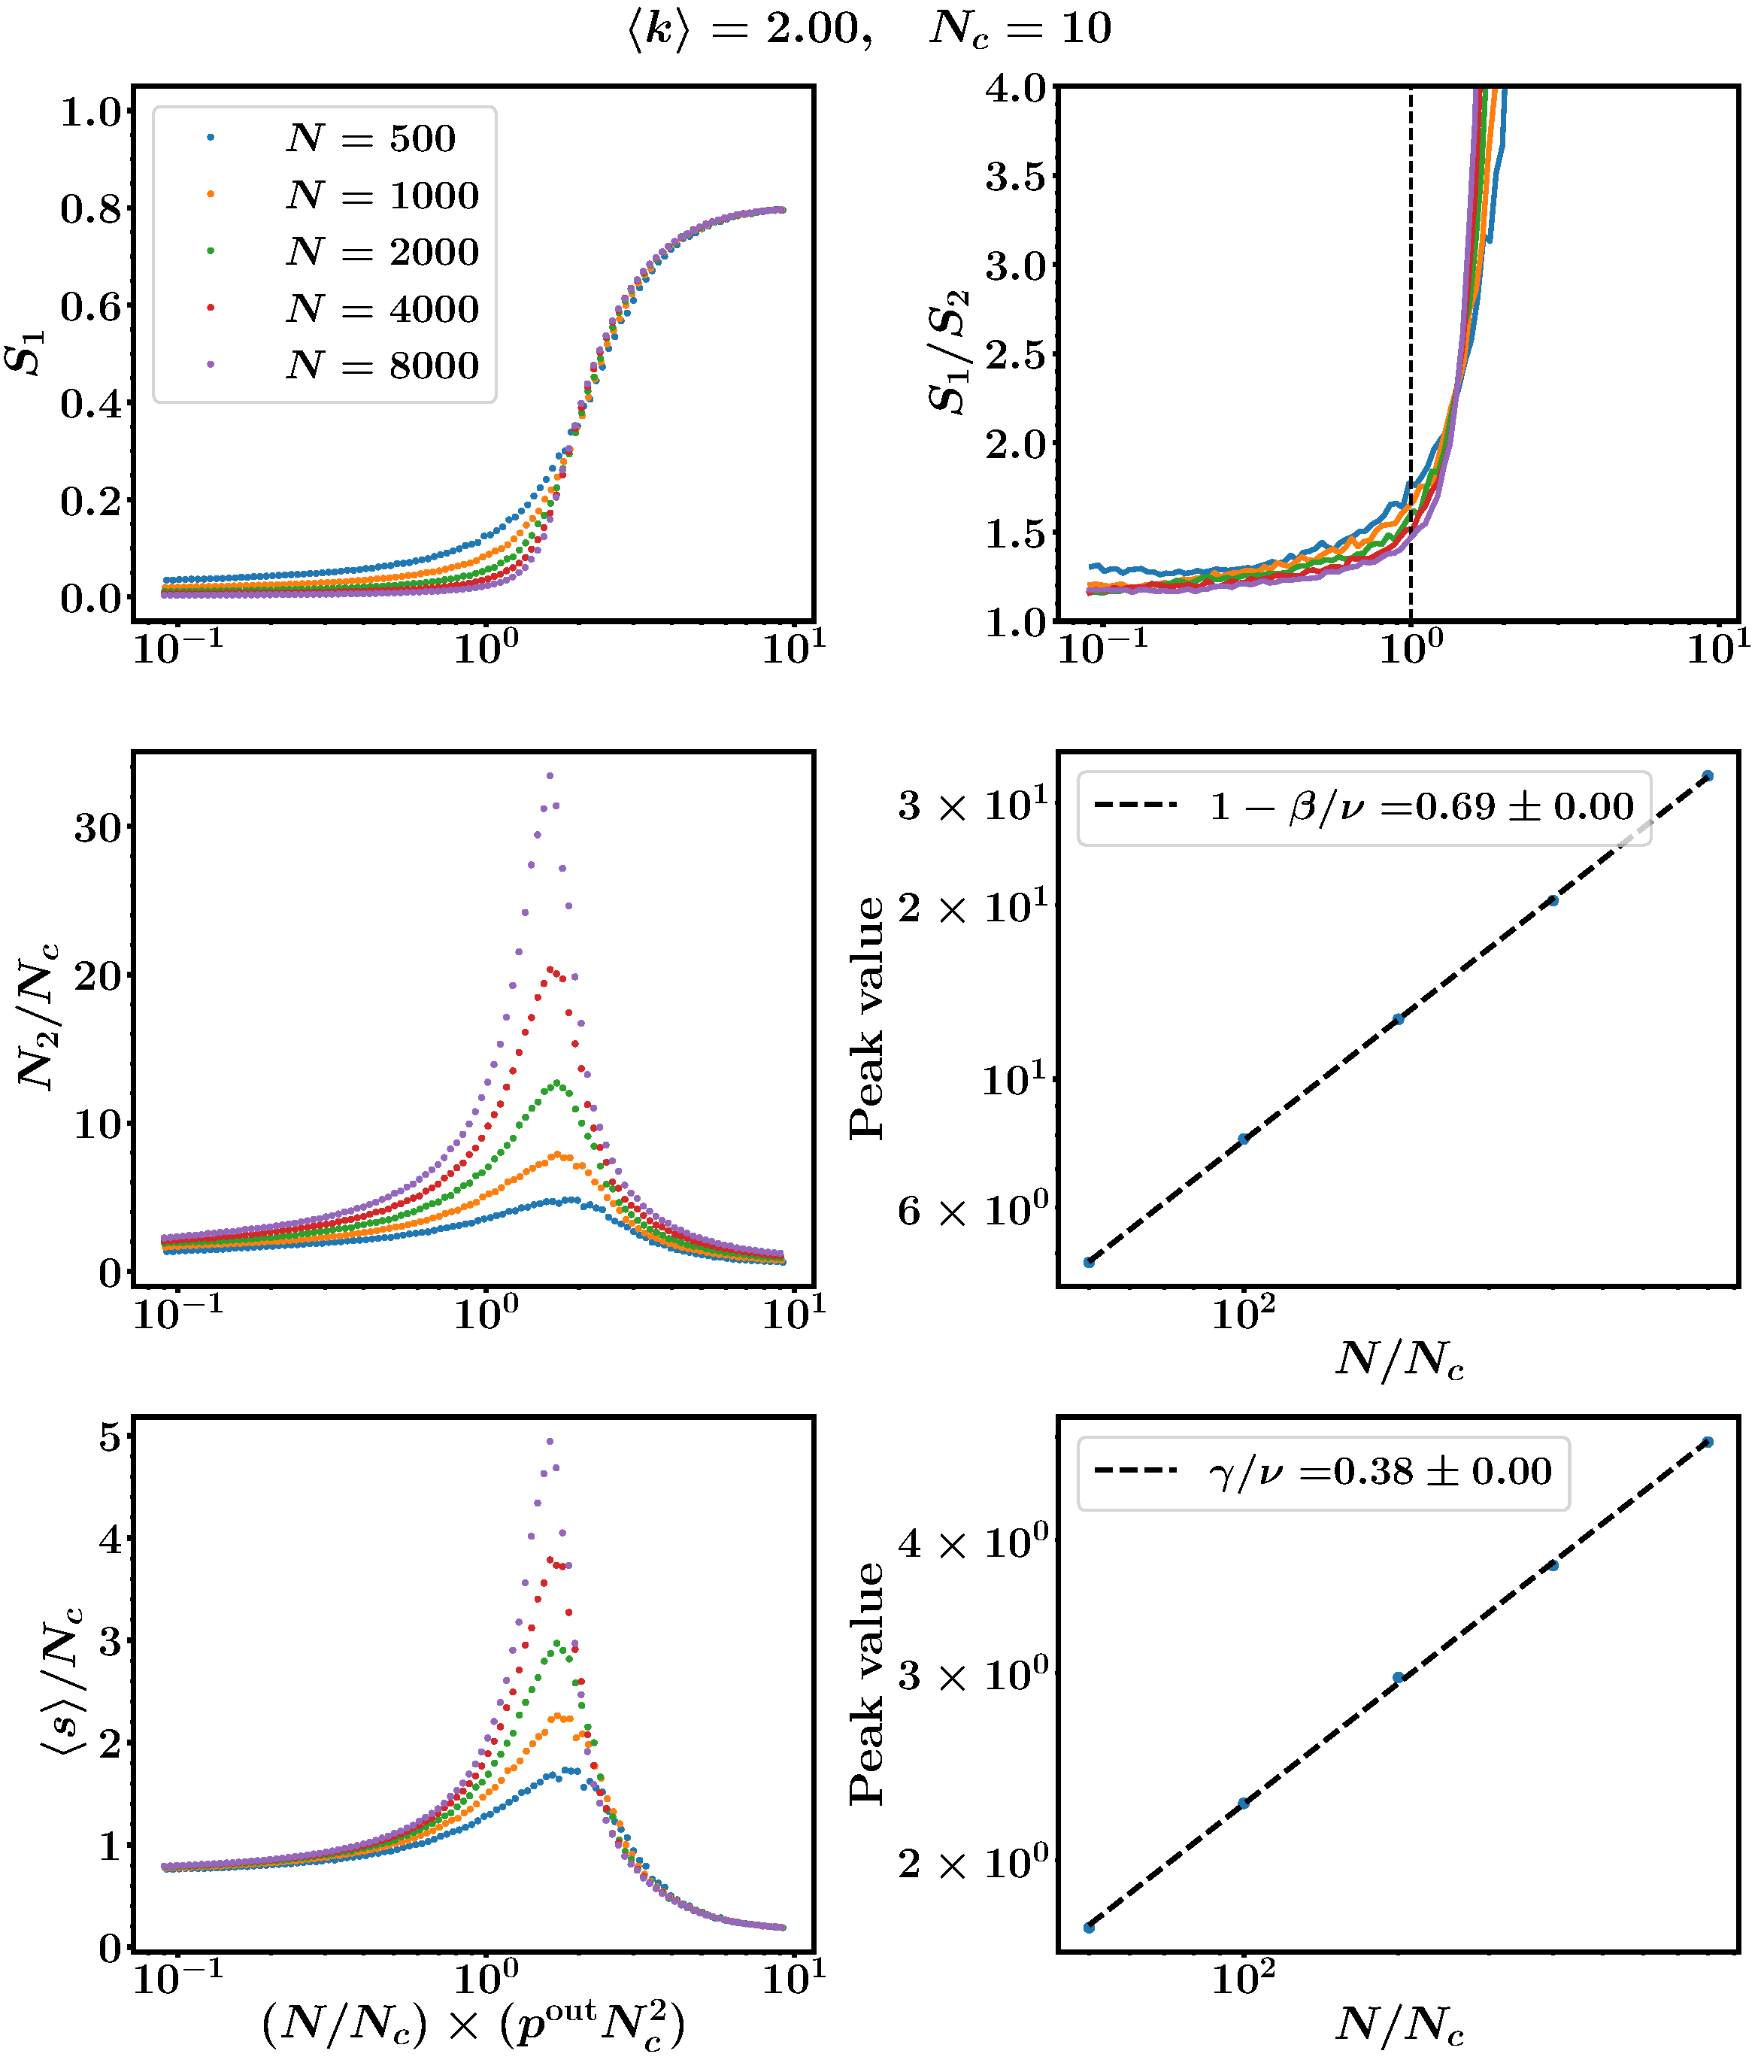
\includegraphics[scale=0.24]{{figures/scaling_k2.00_Nc10_it1000_samples100_Log}.pdf}%
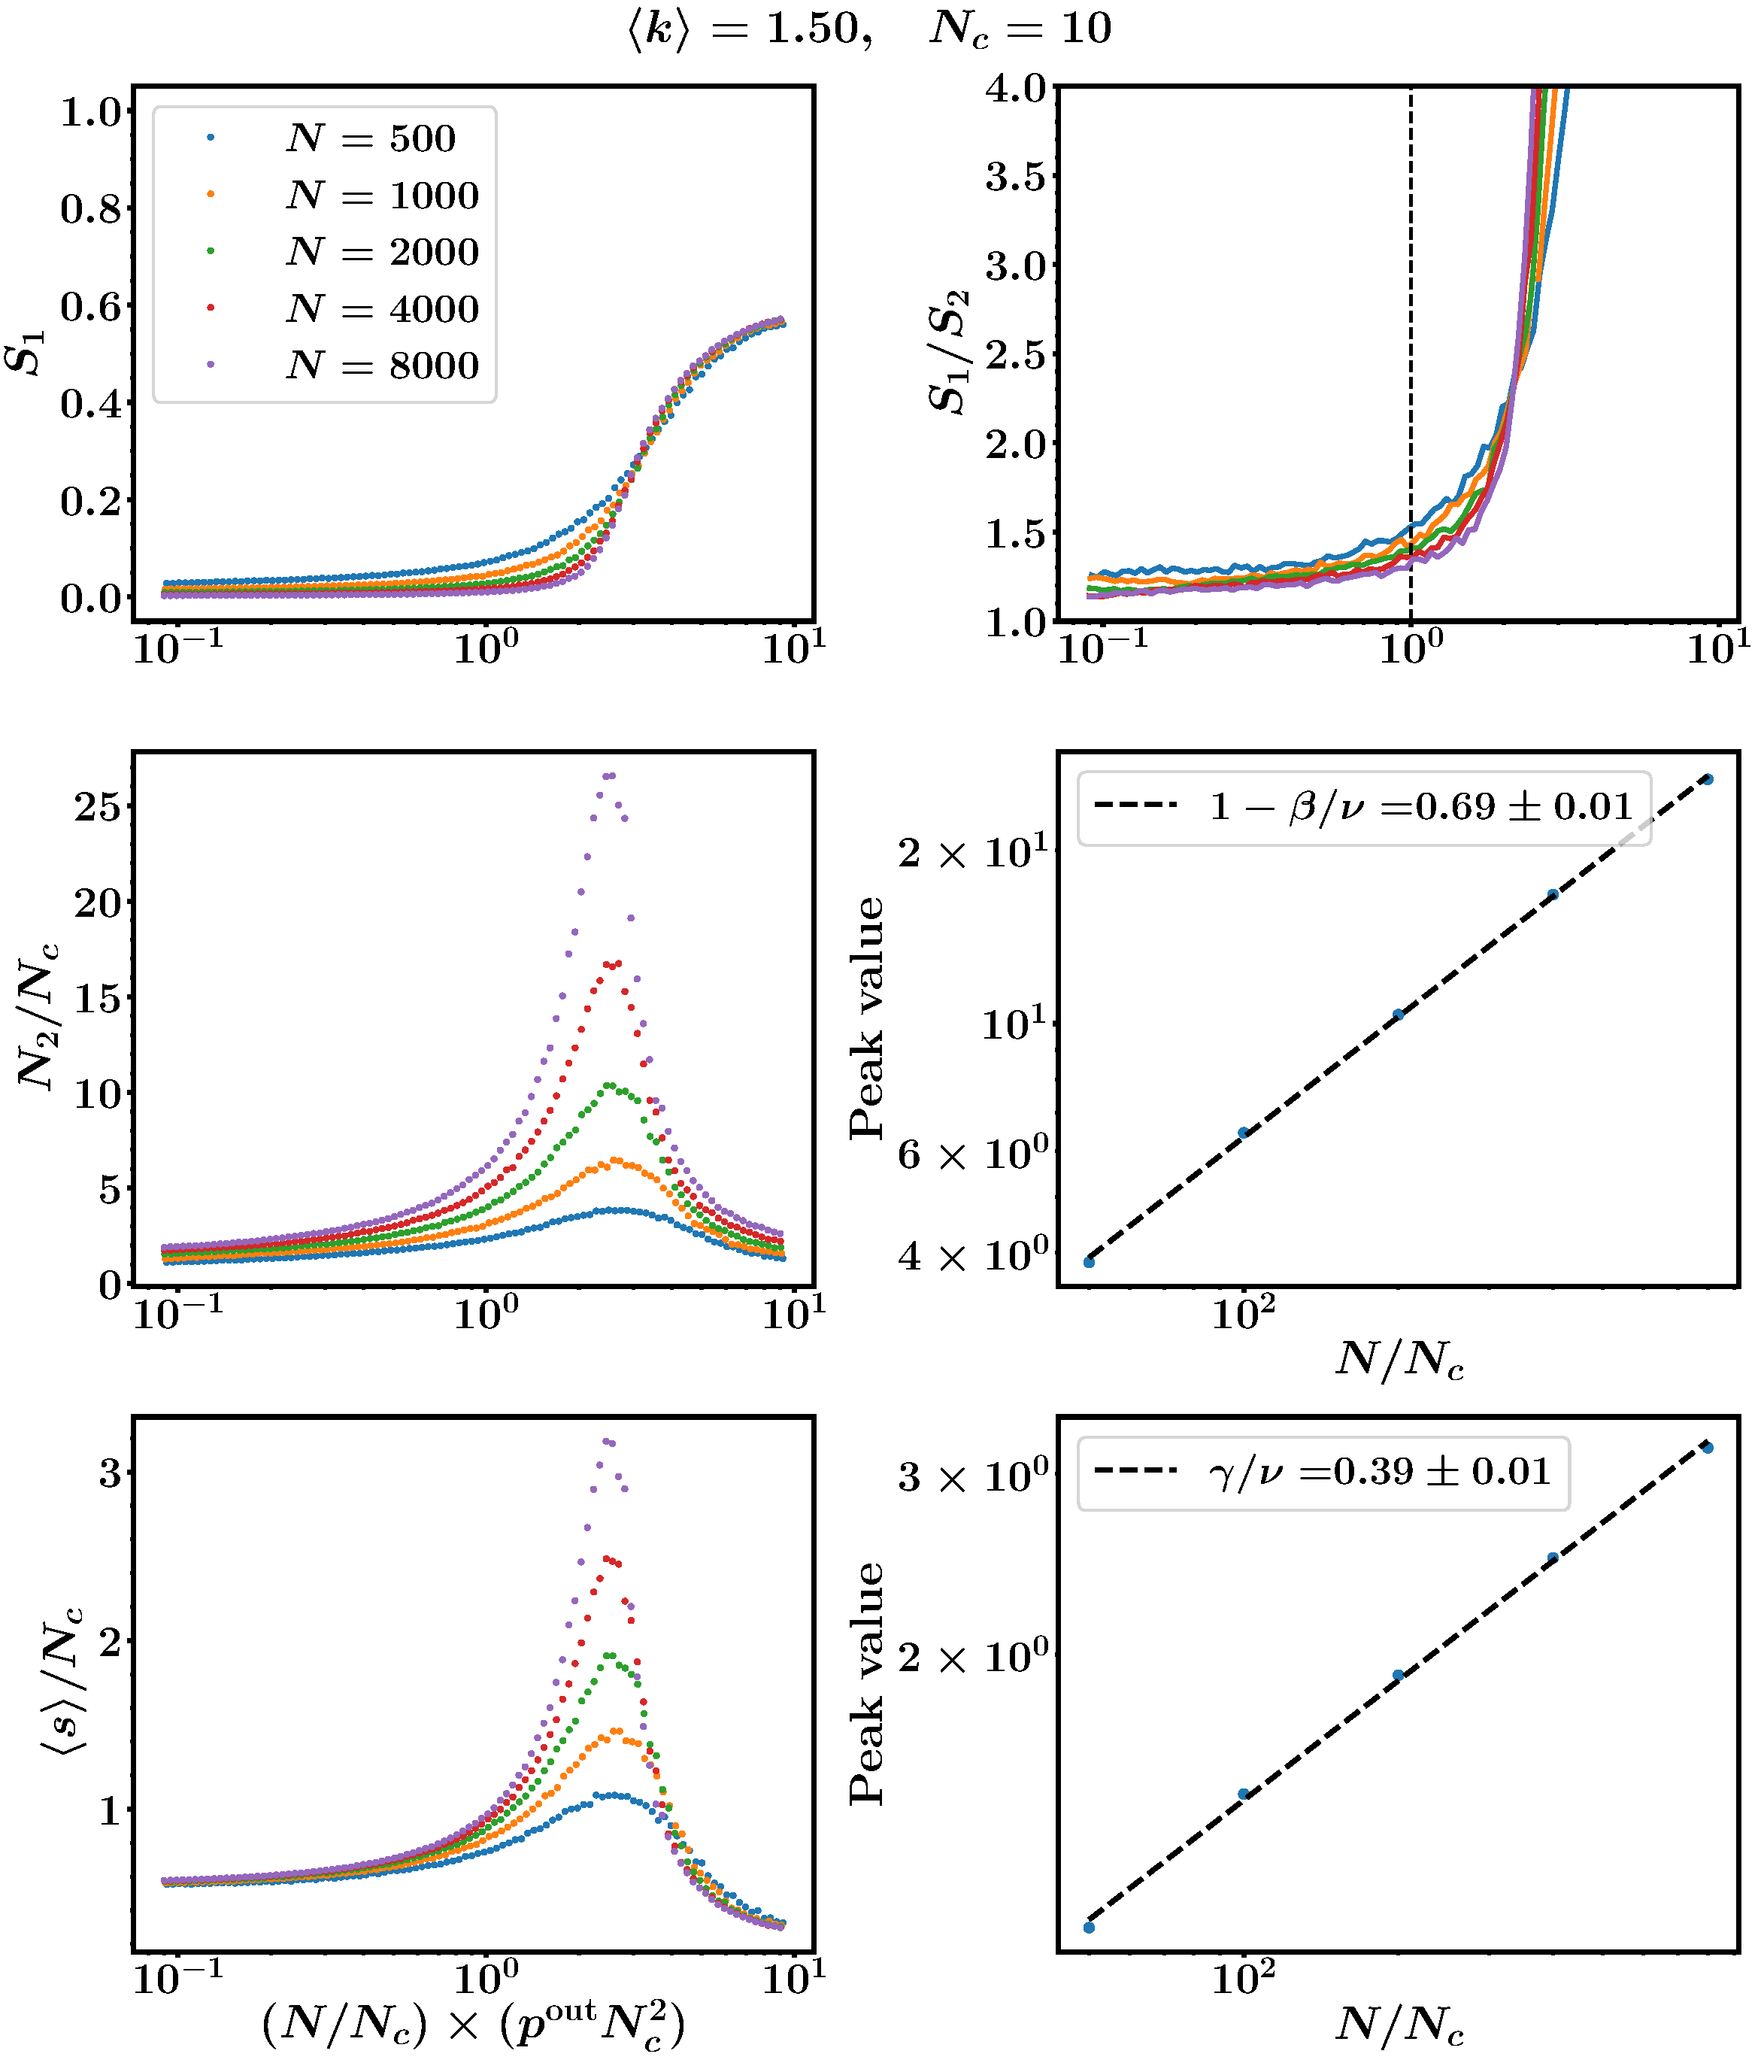
\includegraphics[scale=0.24]{{figures/scaling_k1.50_Nc10_it1000_samples100_Log}.pdf}
\caption{\label{fig:scaling} Scaling of the percolation transition for different values of $\meank$.}
\end{figure}

\begin{figure}
\centering
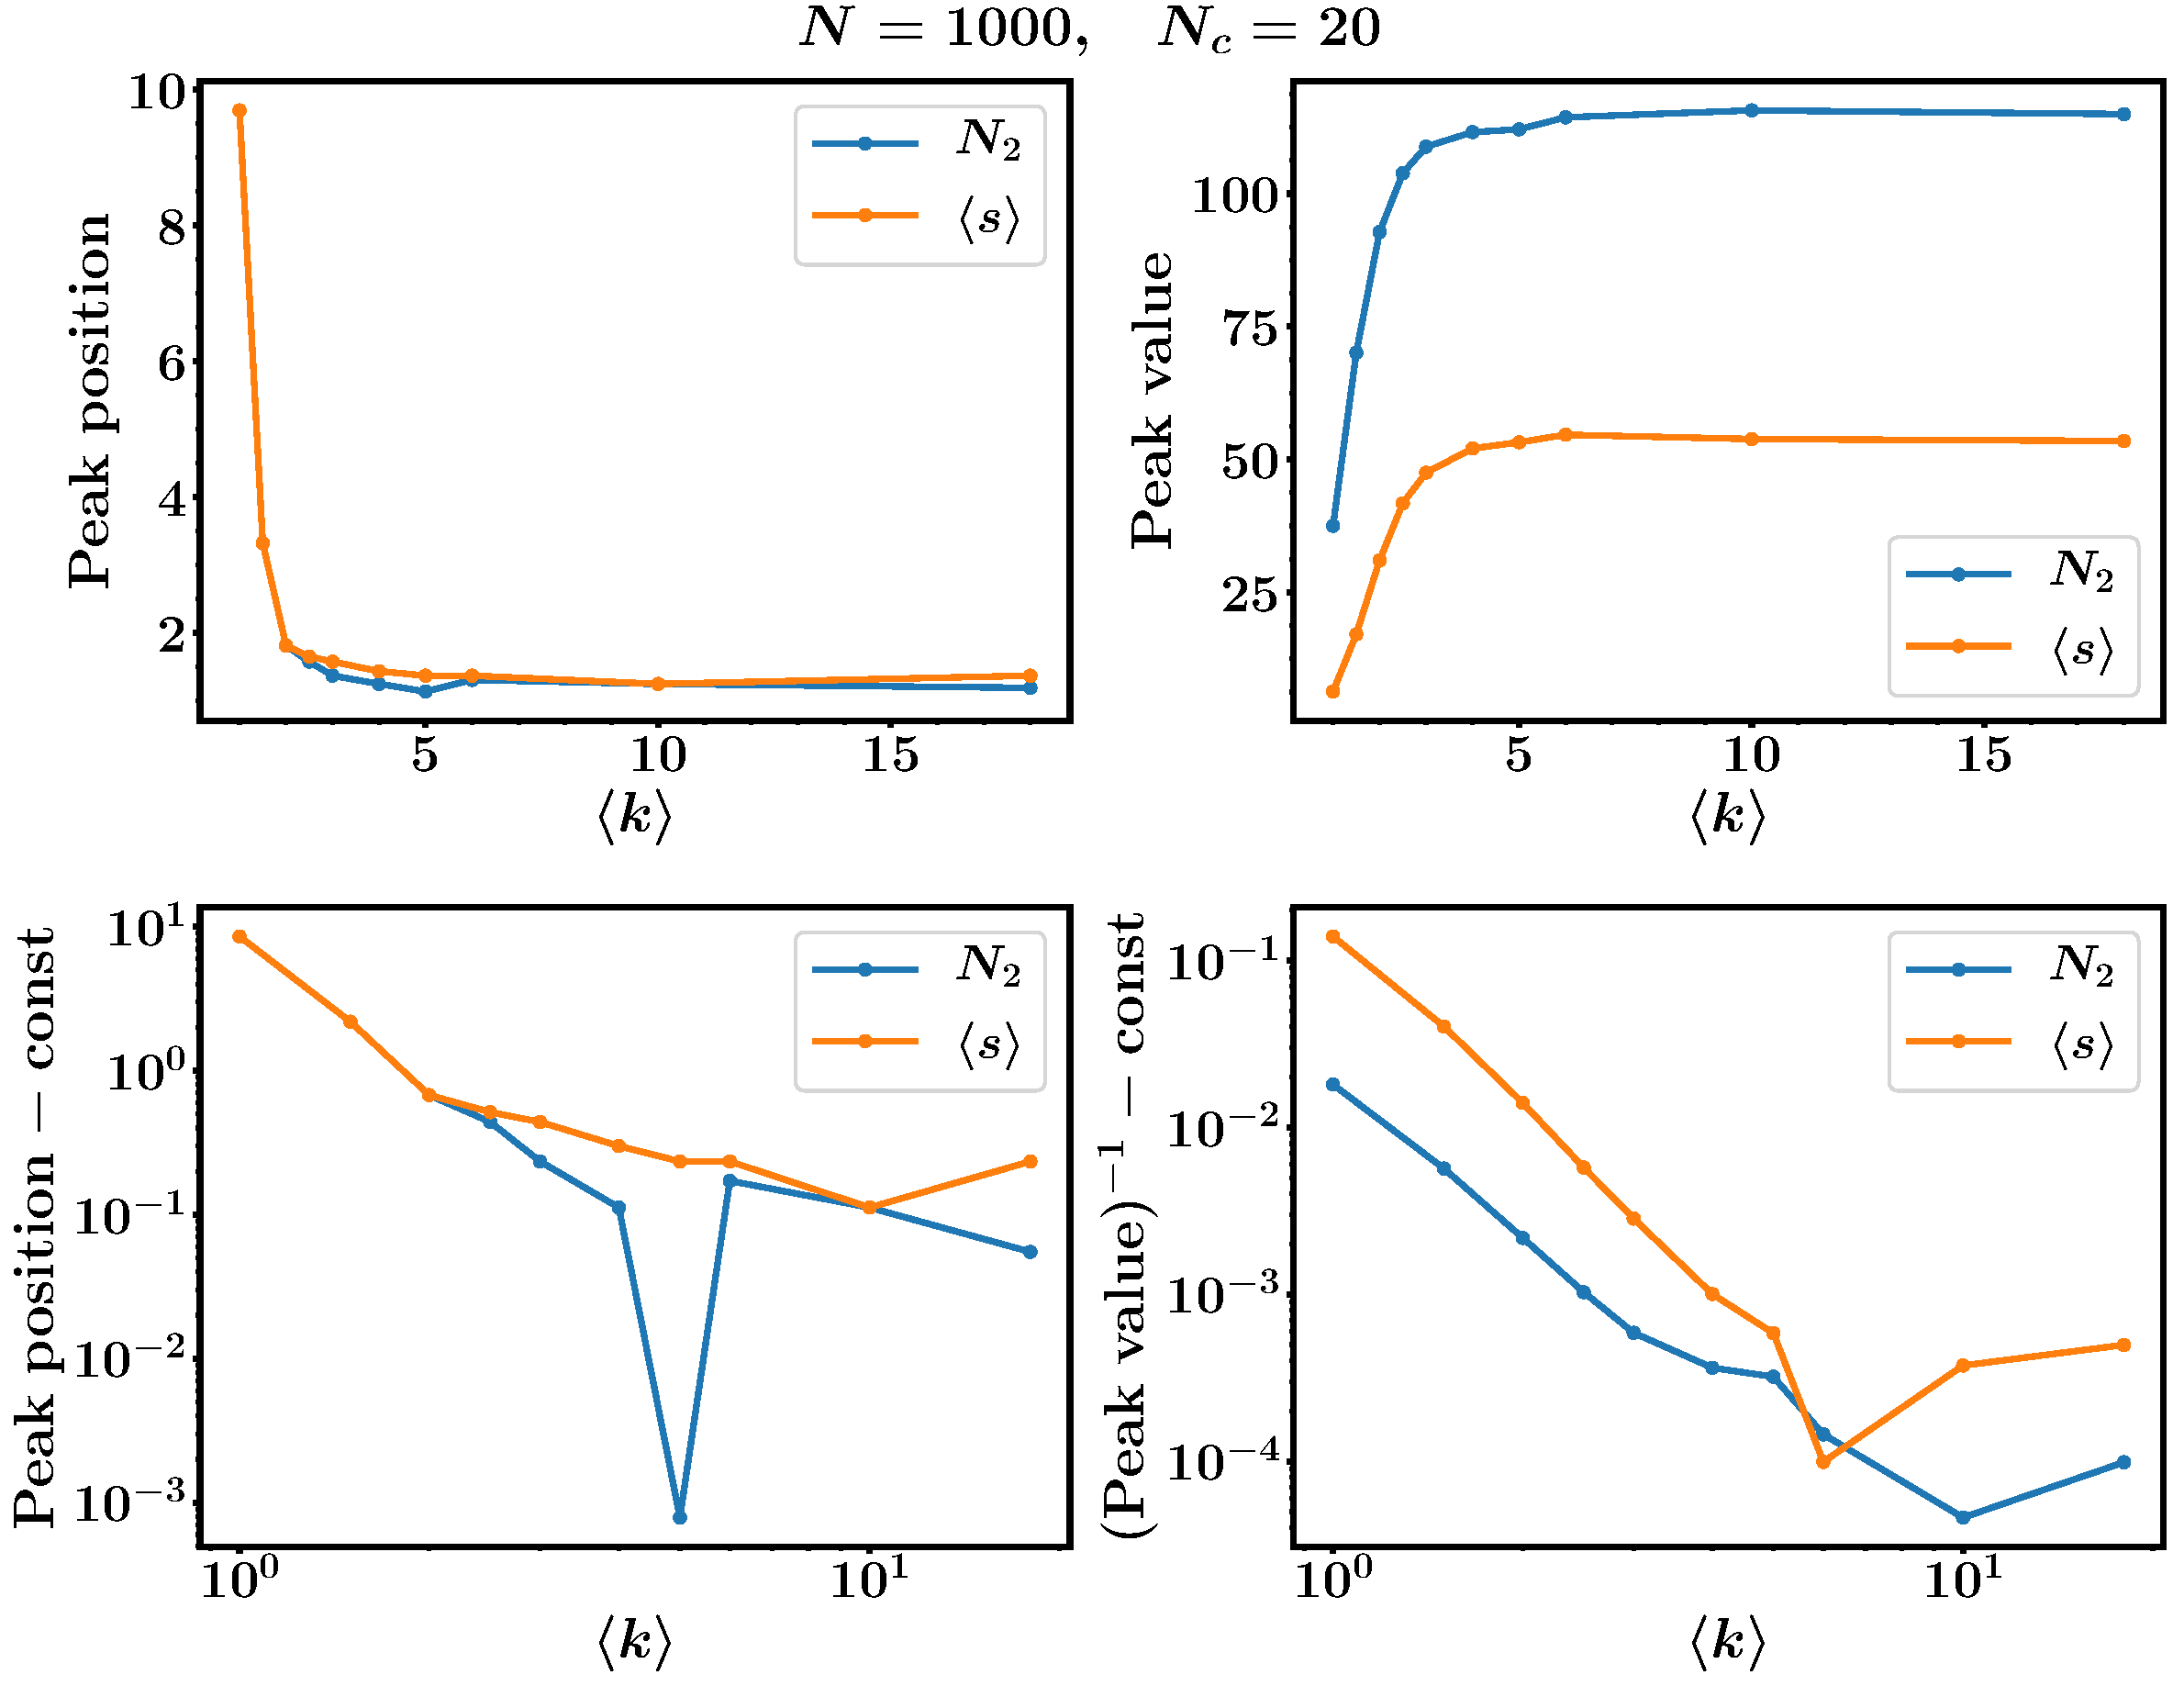
\includegraphics[scale=0.3]{{figures/perc_point_N1000_Nc20_it1000_samples100_Log}.pdf}
\caption{\label{fig:perc_point} Variation of the (finite-size) percolation threshold and size of the susceptibility peak with $\meank$. }
\end{figure}






\end{document}